\documentclass{article}
\usepackage{listings}
\usepackage[margin=1in]{geometry}
\usepackage{graphicx}

\title{CMOR 421/521, Homework \#1: \LaTeX{} Submission}
\author{\texttt{amc50}}
\date{March 7, 2024}

\begin{document}
\maketitle

\section{Compilation}

\subsection{Accessing NOTS Cluster}
It is important to note that the following process is done on Rice Owls Network. This is the case as the cluster login requires accessing through a Secure Shell on the Rice campus network.

\bigskip
\noindent Command used to ssh into NOTS:

\begin{verbatim}
MacBook-Pro-95:cmor-421-521-submissions antoniocrivello$ ssh amc50@nots.rice.edu
\end{verbatim}

\bigskip
\noindent Command used to activate interactive node on NOTS:
\begin{verbatim}
[amc50@nlogin1 ~]$ srun --pty --partition=interactive --ntasks=1 --mem=1G --time=00:30:00 $SHELL
\end{verbatim}

\bigskip
\noindent Command used to load modules needed for compilation:
\begin{verbatim}
[amc50@bc9u7n1 ~]$ module load GCC/13.1.0 
\end{verbatim}

\bigskip
\noindent To access files created on local desktop, a GitHub repository is used. As such, this repository must be cloned on the cluster. This process requires a password-protected key.

\bigskip
\noindent Command used to generate SSH key :
\begin{verbatim}
[amc50@bc9u7n1 ~]$ ssh-keygen -t ed25519 -C "amc50@rice.edu"
\end{verbatim}

\bigskip
\noindent Command used to access public key:
\begin{verbatim}
[amc50@bc9u7n1 ~]$ emacs ~/.ssh/id_ed25519.pub 
\end{verbatim}

\bigskip
\noindent After accessing the SSH key, it is added to list of SSH keys on GitHub.

\bigskip
\noindent Command used to clone cmor-421-521-submission GitHub repository:
\begin{verbatim}
[amc50@bc9u7n1 ~]$ git clone git@github.com:AntonioCrivello/cmor-421-521-submissions.git    
\end{verbatim}

\bigskip
\noindent For compilation on the NOTS Cluster I am utilizing a Makefile. 

\bigskip
\noindent Set of commands to compile project: 
\begin{verbatim}
[amc50@bc9u7n1 homework-1]$ make clean
rm -rf matmul_recursive 

[amc50@bc9u7n1 homework-1]$ make
g++ main.cpp -O3 -std=c++11 -o matmul_recursive
\end{verbatim}

\bigskip
\noindent In order to efficiently generate timings for matrix sizes of $2^{i}$ for i = 4,5,6 ... 10, I have created a bash script to run the aforementioned make clean and make commands with the matrix size as an argument. Additionally, to determine the optimal block size for the block size dependent matrix-matrix multiplication methods these are also supplied as an argument to the executable. After initial testing it was observed that block sizes that are too large exhibited no improvement in the methods. For this reason block sizes above 256 are excluded from the rest of the report.

\bigskip
\noindent Command used to generate timings and compile project:
\begin{verbatim}
[amc50@bc9u7n1 homework-1]$ ./generate-timings.sh 
\end{verbatim}

\section{Matrix-Matrix Multiplication}

\subsection{Column Major Storage for Matrix-Matrix Multiplication}
If the matrix was stored in column major format instead of row major format for matrix-matrix multiplication a few changes should be made. The first is to change how the memory is accessed during the implementation. With row major storage the memory is efficiently access by looping through the rows and then the columns. For the column major formatting, this should be changed, looping through the column first and then the row. This will allow the required data values to be located adjacent to each other. There is also a benefit in unrolling the innermost loop to reduce overhead and utilize the
location of the column values.

\subsection{Matrix Transpose}

For matrices stored in column major format it is expected that $A^{T}B$ would be faster than AB. The primary reason this is the case is because when applying the transpose to matrix A and then multiplying to matrix B, the matrix-matrix multiplication involves looping through the rows of $A^{T}$ and the columns of B. Given then that A is stored in column major format, the transpose of the columns is the rows so the memory accessing will be contiguous. This is an improvement over the noncontiguous accessing that is required for row major containing. 

\section{Optimizing Matrix-Matrix Multiplication}

\subsection{Timing}
\begin{table}[ht!]
    \caption{Naive Matrix-Matrix Multiplication Timings (Seconds) on NOTS}
    \centering
    \resizebox{\textwidth}{!}{%
    \begin{tabular}{|c|c|c|c|c|c|c|c|}
        \hline
        \multicolumn{1}{|c|}{} & \multicolumn{7}{c|}{Block Size} \\
        \cline{2-8}
        \multicolumn{1}{|c|}{Matrix Size} & 4 & 8 & 16 & 32 & 64 & 128 & 256 \\
        \hline
        n = 16 & 3.10545e-06 & 3.10125e-06 & 3.08615e-06 & & & & \\
        \hline
        n = 32 & 2.54184e-05 & 2.49542e-05 & 2.42004e-05 & 2.51914e-05 & & & \\
        \hline
        n = 64 & 0.000201979 & 0.00019916 & 0.000201801 & 0.000199571 & 0.000211543 & & \\
        \hline
        n = 128 & 0.00200881 & 0.00199386 & 0.00203293 & 0.00199047 & 0.00208364 & 0.00199213 & \\
        \hline
        n = 256 & 0.0290755 & 0.028877 & 0.0289425 & 0.0287296 & 0.0286273 & 0.0280176 & 0.0283625 \\
        \hline
        n = 512 & 0.233694 & 0.233261 & 0.233572 & 0.233511 & 0.2335 & 0.233596 & 0.233555 \\
        \hline 
        n = 1024 & 1.85073 & 1.88143 & 1.85181 & 1.85074 & 1.84941 & 1.844 & 1.85132 \\
        \hline
    \end{tabular}
    }
\end{table}

\subsection{Timing}
\begin{table}[ht!]
    \caption{Blocked Matrix-Matrix Multiplication Timings (Seconds) on NOTS}
    \centering
    \resizebox{\textwidth}{!}{%
    \begin{tabular}{|c|c|c|c|c|c|c|c|}
        \hline
        \multicolumn{1}{|c|}{} & \multicolumn{7}{c|}{Block Size} \\
        \cline{2-8}
        \multicolumn{1}{|c|}{Matrix Size} & 4 & 8 & 16 & 32 & 64 & 128 & 256 \\
        \hline
        n = 16 & 4.285e-06 & 3.08285e-06 & 3.18565e-06 & & & & \\
        \hline
        n = 32 & 3.27257e-05 & 2.49542e-05 & 2.42004e-05 & 2.51914e-05 & & & \\
        \hline
        n = 64 & 0.000248281 & 0.00019916 & 0.000201801 & 0.000199571 & 0.000211543 & & \\
        \hline
        n = 128 & 0.00193728 & 0.0014215 & 0.00131316 & 0.00143792 & 0.00210973 & 0.00189773 & \\
        \hline
        n = 256 & 0.0185984 & 0.0118275 & 0.0111113 & 0.0151655 & 0.015999 & 0.020307 & 0.0279572 \\
        \hline
        n = 512 & 0.155723 & 0.103269 & 0.113957 & 0.164497 & 0.216412 & 0.228384 & 0.232447 \\
        \hline
        n = 1024 & 1.20218 & 0.845138 & 0.892962 & 1.25336 & 1.91301 & 1.87324 & 1.85621 \\
        \hline
    \end{tabular}
    }
\end{table}


\subsection{Discussion}

As seen in Table 2, the block size is independent of the size of the matrix. This is to be expected as the purpose of the Blocked Matrix-Matrix method is to take advantage of the machine's cache. By dividing the matrix of size n into N sub-matrices that fit into the fast memory this is possible. As such, the optimal block size is dependent on how large the fast memory is rather than how large the matrix is. The optimal block sized based on the timings is b = 8.

\subsection{Roofline Plot Results}

For the following roofline plot, the operations are run using the NOTS Cluster Intel(R) Xeon(R) CPU E5-2650 v2 @ 2.60Hz. For this specific processor the CPU specifications are a max performance of 166.4 GFLOPS and max memory bandwidth of 59.7 GB/s. For this  model only the performance for one core will be considered, as such with 8 cores the peak performance per core is 20.8 GFLOPS. To determine the theoretical limit, the roofline is defined as min(peak performance, CI * peak bandwidth), where CI is the computational intensity. 

\noindent For the naive implementation, plotting the method's performance involves determining the CI, using equation (1). Additionally, the GFLOPS/s is calculated by using the experimentally measured run times. The blocked method is evaluated similarly, however, now uses the CI defined by (2). In this equation b is the block size, used to tile the matrix. 

UNITS CHECK

\begin{equation}
CI = \frac{2 \cdot n^{3}}{(3 \cdot n^{2} + n^{3}) * 8}
\end{equation}

\begin{equation}
CI = \frac{2 \cdot n^{3}}{(2 \cdot n^{2} + \frac{2 \cdot n^{3}}{b}) * 8}
\end{equation}

\begin{figure}[!htb]
    \centering
    \fbox{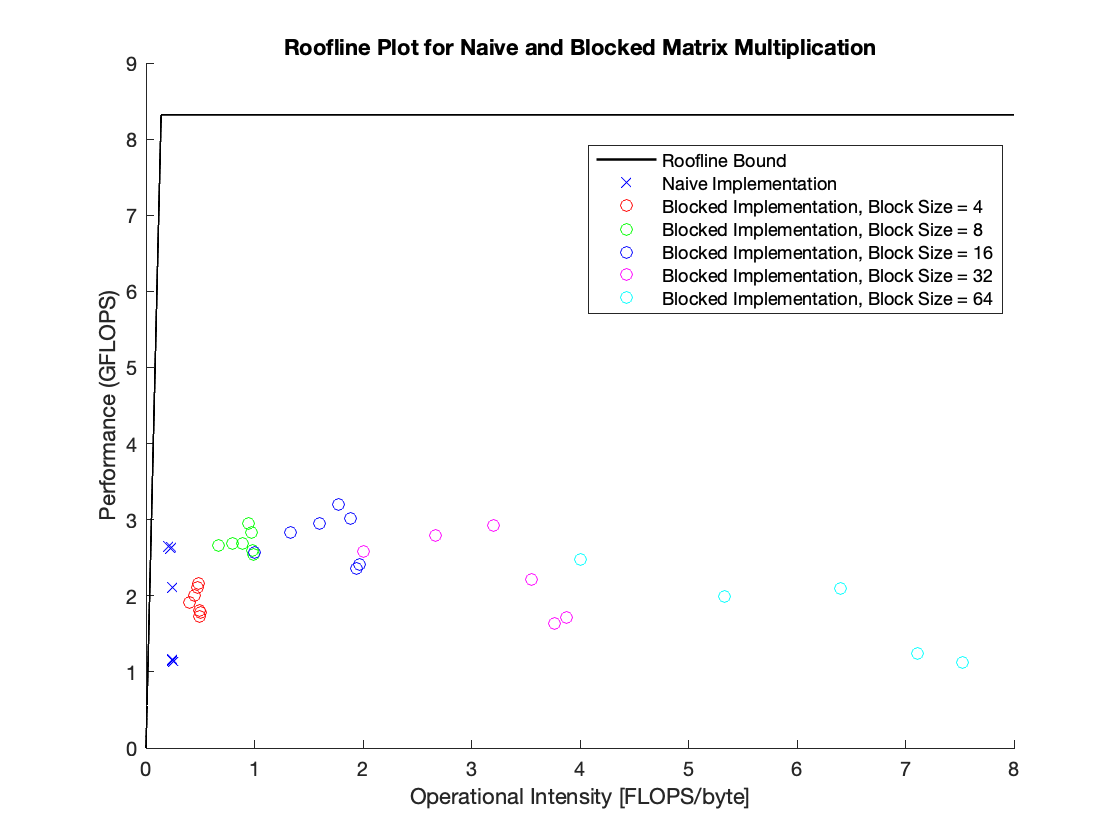
\includegraphics[width=0.8\linewidth]{roofline_v1.png}}
    \caption{Roofline Plot for Naive and Blocked Matrix-Matrix Multiplication}
\end{figure}

\section{Recursive Matrix-Matrix Multiplication}

In my implementation I have two versions of Recursive Matrix-Matrix multiplication. In the first version when running the "microkernel" if the matrix is smaller than the block size, not intermediate doubles are allocated. Instead, the writing to memory for C matrix is done at the inner loop every time. The second version, instead, allocated doubles and then writes to C at the end of the second inner loop. The difference in performance is not substantial but is still interesting.

\subsection{Timing}
\begin{table}[ht!]
    \caption{Recursive Matrix-Matrix Multiplication Timings (Seconds) on NOTS}
    \centering
    \resizebox{\textwidth}{!}{%
    \begin{tabular}{|c|c|c|c|c|c|c|c|}
        \hline
        \multicolumn{1}{|c|}{} & \multicolumn{7}{c|}{Block Size} \\
        \cline{2-8}
        \multicolumn{1}{|c|}{Matrix Size} & 4 & 8 & 16 & 32 & 64 & 128 & 256 \\

        \hline
        n = 16 & 4.3746e-06 & 3.84855e-06 & 4.0144e-06 & & & & \\
        \hline
        n = 32 & 3.59681e-05 & 2.93144e-05 & 2.83537e-05 & 2.9477e-05 & & & \\
        \hline
        n = 64 & 0.000267287 & 0.000220274 & 0.000219527 & 0.000221825 & 0.000280406 & & \\
        \hline
        n = 128 & 0.00216819 & 0.00225175 & 0.00230736 & 0.00247268 & 0.00291227 & 0.00292425 & \\
        \hline
        n = 256 & 0.0188836 & 0.0194226 & 0.0213402 & 0.0266196 & 0.0287319 & 0.0306485 & 0.034413 \\
        \hline
        n = 512 & 0.172686 & 0.180409 & 0.24999 & 0.304377 & 0.328572 & 0.350685 & 0.327068 \\
        \hline
        n = 1024 & 1.35766 & 1.44219 & 2.00194 & 2.38584 & 2.58745 & 2.60176 & 2.6445 \\
        \hline
    \end{tabular}
    }
\end{table}

\begin{table}[ht!]
    \caption{Recursive with Intermediates Matrix-Matrix Multiplication Timings (Seconds) on NOTS}
    \centering
    \resizebox{\textwidth}{!}{%
    \begin{tabular}{|c|c|c|c|c|c|c|c|}
        \hline
        \multicolumn{1}{|c|}{} & \multicolumn{7}{c|}{Block Size} \\
        \cline{2-8}
        \multicolumn{1}{|c|}{Matrix Size} & 4 & 8 & 16 & 32 & 64 & 128 & 256 \\
        \hline
        n = 16 & 4.3127e-06 & 3.8545e-06 & 3.1154e-06 & & & & \\
        \hline
        n = 32 & 3.30702e-05 & 2.88791e-05 & 3.02864e-05 & 2.44447e-05 & & & \\
        \hline
        n = 64 & 0.000264601 & 0.000217845 & 0.00021575 & 0.000218845 & 0.000211155 & & \\
        \hline
        n = 128 & 0.00218899 & 0.00223674 & 0.00228827 & 0.00244738 & 0.00292257 & 0.00191426 & \\
        \hline
        n = 256 & 0.0196593 & 0.0194059 & 0.0213406 & 0.0274662 & 0.0288066 & 0.0306233 & 0.0279678 \\
        \hline
        n = 512 & 0.172776 & 0.180293 & 0.249874 & 0.304238 & 0.328168 & 0.350561 & 0.326953 \\
        \hline
        n = 1024 & 1.35529 & 1.41505 & 1.98208 & 2.38522 & 2.58701 & 2.60168 & 2.75475 \\
        \hline
    \end{tabular}
    }
\end{table}

\subsection{Optimizing Recursive Matrix-Matrix Multiplication}
For the Recursive Matrix-Matrix Multiplication method, the optimal block size is 8, which is the same as the Blocked Matrix-Matrix multiplication method. Given that these methods are run on the same CPU with the same fast cache this makes sense. It is important to note that the optimal block size does slightly vary between 8 and 16, but this could be an artifact of inconsistent timings.

\subsection{Implementation Check}
In order to confirm the correctness of the Recursive Matrix-Matrix Multiplication method, matrices \( A \) and \( B \) are initialized to the identity matrix. The matrices are then multiplied together, and the resulting matrix \( C \) is expected to be equal to the identity matrix \( I \). To verify that \( C \) is indeed equal to \( I \) up to machine precision, an elementwise comparison is performed, and the absolute difference between corresponding elements of \( C \) and \( I \) is computed. These differences are accumulated, and if the sum exceeds \( 1 \times 10^{-14} \times n \), where \( n \) is the size of the matrix, it indicates that the matrices are not identical. It is important to note that the scaling is included due to numerical roundoff. If the sum is within this allowable tolerance, them method has been correctly implemented. In my implementation, this equality check is performed after each call of a matrix-matrix multiplication function.

\subsection{Roofline Plot Results}

\begin{equation}
CI = \frac{2}{3 * 8} \cdot b 
\end{equation}

\begin{figure}[!htb]
    \centering
    \fbox{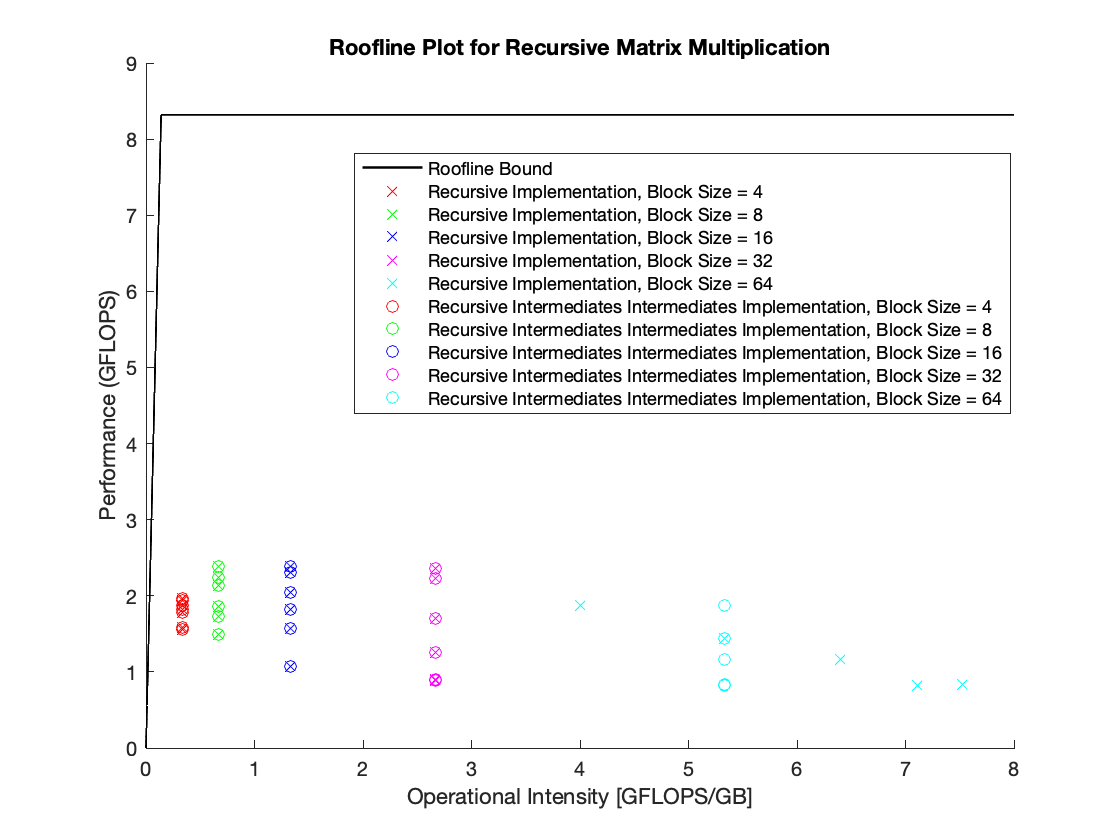
\includegraphics[width=0.8\linewidth]{recursive_v1.png}}
    \caption{Roofline Plot for Recursive Matrix-Matrix Multiplication}
\end{figure}

\subsection{Discussion}
The performance of the Recursive Matrix-Matrix multiplication method was outperformed by that of optimized Blocked Matrix-Matrix multiplication. There are a few reasons this could be the case. The most likely source of the reduced performance is the additional overhead resulting from eight function calls per recursion. This is in comparison to looping over the iterations.

\noindent As expected there was not much difference between the two recursive methods. There was a slight improved speed from the intermediates version for larger matrix sizes, but that difference was even less for small matrices.

\end{document}

